% !TeX spellcheck = en_US
\chapter{Introduction}\label{intro}

\section{The revelation of the HPV}
%Algo importante que contar
One of the biggest scientific discoveries in the past 30 years was the connection between HPV infection of the cervix and cervical cancer. This achievement resulted from the original seminal findings by Harald zur Hausen and his group, they found that human papillomavirus genotype 16 can be detected in cervical cancer tissue. 
\begin{figure}[ht]
	\centering
	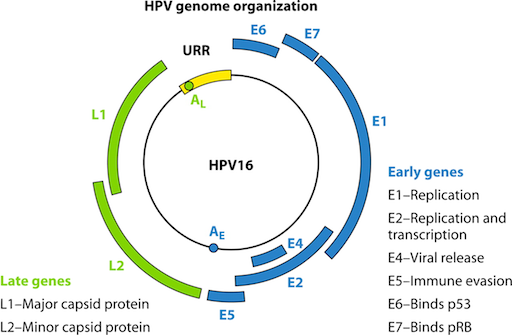
\includegraphics[scale=0.7]{IMG/genoma.png}
	\caption{Graphic illustrating the genomic organization of a typical mucosal high-risk HPV. The genome contains early (E) and late regions (L), which relate to the positions of the genes within the genome and their timing of expression during the viral life cycle. The early (E) region carries a number of genes which function at the level of viral replication and transcription, i.e., E2, E1, E6, and E7. E2 encodes a protein which has an auxiliary role in viral replication and also functions at the level of transcriptional regulation of the viral early genes. The E6 and E7 genes encode the major transforming proteins of the oncogenic HPVs. The late region (L) encodes viral structural proteins, with L1 being the major capsid protein and L2 being the minor capsid protein, adopted from 
	\cite{Stanley215}.}
	\label{genoma}
\end{figure}

The finding was followed by epidemiologists, molecular biologists, vaccinologists, and clinicians culminating in 2006 with the development of effective prophylactic vaccines for HPV, which have the means to prevent 70-80\% of cervical cancers \cite{olsen2015revisiting}. Zur Hausen was awarded the Nobel Prize in Physiology or Medicine in 2008, in recognition of his discovery.

\begin{figure}[ht]
	\centering
	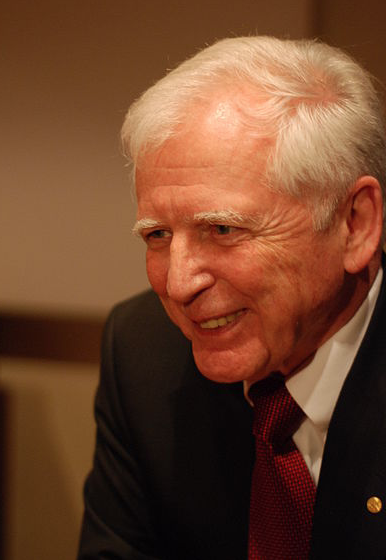
\includegraphics[scale=0.7]{IMG/zurHausen.png}
	\caption{Harald zur Hausen (born 11 March 1936) is a German virologist and professor emeritus. He has done research on cancer of the cervix, where he discovered the role of papilloma viruses, for which he received the Nobel Prize in Physiology or Medicine 2008. Adopted from \cite{haraldZur2010}}
	\label{zurHausen}
\end{figure} 
%Foto de Zur Hausen

% La ETS mas común del mundo
With more than 600 million cases worldwide, including 20 million in the United States, HPV is the most common STD, according to the Centers for Disease Control and Prevention (CDC) and the World Health Organization (WHO). More than 40 HPV types can infect the genital areas of men and women, including the skin of the penis, vulva, and anus, and the linings of the vagina, cervix, and rectum.

Most people who become infected with HPV do not know they have it. Usually, the body's immune system gets rid of the HPV infection naturally within two years. This is true of both high risk (HR) and low risk (LR) types. By age 50, at least 4 out of every 5 women will have been infected with HPV at one point in their lives. HPV is also very common in men, and often has no symptoms.

%Datos de lo malo que es
HPV types are often referred to as LR wart causing or HR cancer causing \cite{Clifford1157}, based on whether they put a person at risk for cancer. The types of HPV that can cause genital warts (GW) are not the same as the types that can cause cancer. Persistent HPV infections with genotypes 16 and 18 are responsible for about 70\% of all cervical cancer, with 40-85\% of other anogenital cancers: anal, penile, vaginal, and vulvar cancer, and also 16-28\% of the head and neck cancers \cite{olsen2015revisiting}. HPV is a cause of other non malignant diseases, to mention genotypes 6 and 11 cause about 90\% of anogenital warts \cite{lacey2006burden}.

\begin{figure}[ht]
	\centering
	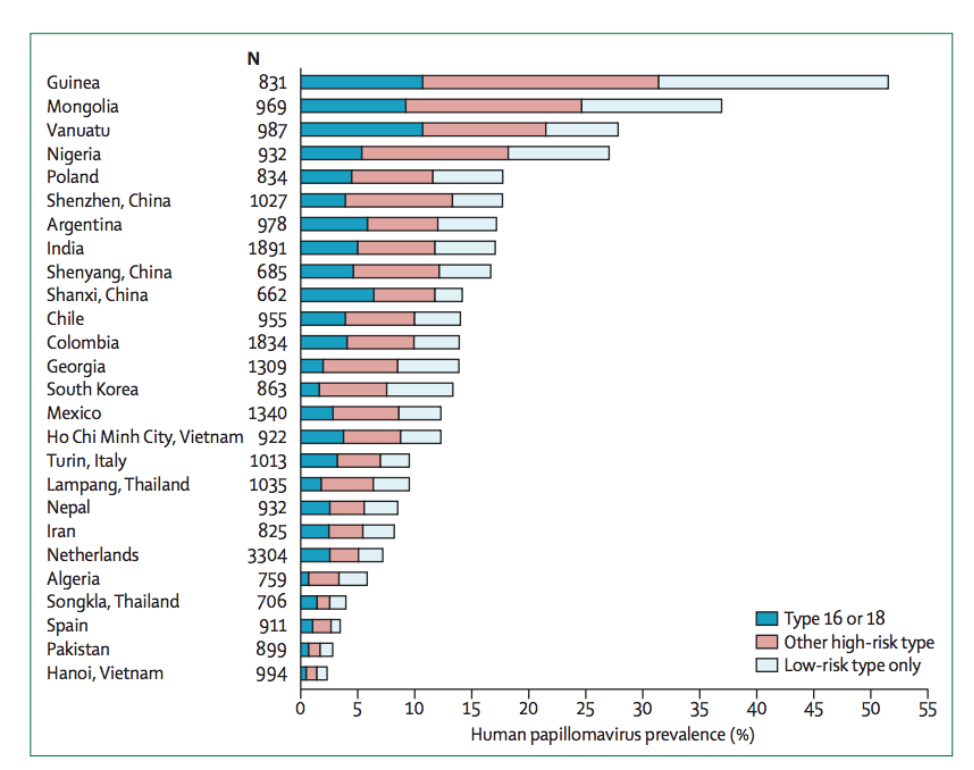
\includegraphics[scale=0.7]{IMG/prevalence.png}
	\caption{Age-adjusted prevalence of cervical human papillomavirus DNA in sexually active women aged 15-69 years. Data are from IARC Prevalence Surveys, 1990-2012, adopted from \cite{Marx1986HumanPV}.}
	\label{ageAdjusted}
\end{figure} 
%Foto de prevalencia

%Lo que cuesta $$$$
It is estimated that about 1 million new cases of GW are reported each year and the cost of treatment is increased by the tendency of these warts to recur after initial clearance. The cost of the treatment of GW was estimated to exceed \$ $3.8$ billion in the U.S. in $1997$ \cite{roberts1999vaccine}. In Spain there were $35,000$ cases in women in $2007$ with an overall annual cost of \euro \ $47$ millions \cite{castellsague2012prevalence}.

%Empiezo con las vacunas
\section{Vaccines and mathematical models}

Since the release of the first vaccines in 2006, nowadays there are three available: a quadrivalent (including HPV genotypes 16, 18, 6 and 11) and a bivalent vaccine (including genotypes 16 and 18) and a nonavalent (including genotypes 6, 11, 16, 18, 31, 33, 45, 52 and 58). All vaccines are efficacious to prevent against precancerous lesions in the cervix, vulva or vagina; in addition, the quadrivalent and nonavalent prevent precancerous anal lesions, anal cancer and anogenital warts. 

%Two vaccines consisting of non-infectious HPV virus-like particles (VLP) \cite{mcneil2006invented} containing the capsid protein L1 of the virus but not the viral DNA. They induce a high immune response and prevent premalignant lesions. Both vaccines contain genotypes $16$ and $18$, and one of them adds VLP against genotypes $6$ and $11$ (HPV4).

According to the Advisory Committee on Immunization Practices (ACIP) from the Centers for Disease Control (CDC) and Prevention, new recommendations are given for use of a 2-dose schedule for girls and boys who initiate the vaccination series at ages 9 through 14 years. Three doses remain recommended for persons who initiate the vaccination series at ages 15 through 26 years and for immunocompromised persons.

The HPV vaccine induces a herd immunity effect in genital warts when a large number of the population is vaccinated. This aspect should be taken into account when devising new vaccine strategies, like vaccination at older ages or male vaccination. Numerous cost-effectiveness studies of HPV-vaccination have been published in other countries. However, few studies include the prophylactic effect of all HPV-associated diseases, or the impact of vaccinating men.

%Therefore, it is important to develop mathematical models with good predictive capacities. We devised a sexual contact network that was calibrated to simulate the Spanish epidemiology of different HPV genotypes. Through this model, we simulated the scenario that occurred in Australia in 2007, where 12-13 year-old girls were vaccinated with a three-dose schedule of a vaccine containing genotypes 6 and 11, which protect against genital warts, and also a catch-up program in women up to 26 years of age. Vaccine coverage were $73\%$ in girls with three doses and with coverage rates decreasing with age until $52\%$ for 20-26 year-olds. A fast $59\%$ reduction in the genital warts diagnoses occurred in the model in the first years after the start of the program, similar to what was described in the literature.%

In Spain HPV vaccine is given to adolescent girls as part of the national immunization programme, and is recommended at different age groups in different Autonomous Communities.
In the Region of Valencia, Spain, the vaccine is administered to $< 15$ girls. Similar vaccination strategies of this kind were modeled by Elbasha et al. \cite{elbasha2007model,elbasha2005vaccination} by means of a compartmental model with $17$ age groups for each gender. This model focuses mainly on the development of cervical intraepithelial neoplasia (CIN) and its progression from CIN1 to CIN3. According to these authors vaccination must be implemented for adolescent girls aged between $12$ and $14$ years. Elbasha et al. also found some evidences that the vaccination of boys could also be cost-effective \cite{elbasha2007model}. By vaccinating girls alone a $83\%$ reduction in the incidence of GW is expected but this reduction is increased to $97\%$ if boys are also vaccinated.

It is important to develop mathematical models with good predictive capacities. Some models have shown that the female vaccination program has some herd immunity and the impact of implementing the vaccination in males may not be cost effective. Besides, there is no economic analysis of the nonavalent program in Spain, and it is important from the decision making perspective.

Random network mathematical models may simulate the interactions and propagation of all these viruses through sexual contacts among a population of more than half million people (including heterosexual and homosexual populations). 

Before proceeding with the definition of our model, it is convenient to give a brief and general perspective on the emergent field of network research for the readers not familiar with these techniques and their application in epidemiology. A network is, basically, a model which derives from the abstract mathematical concept of a graph composed by a set of points (the so-called nodes) connected among them by some lines or edges (known as ``links'' in the case of networks).

\begin{figure}[ht]
	\centering
	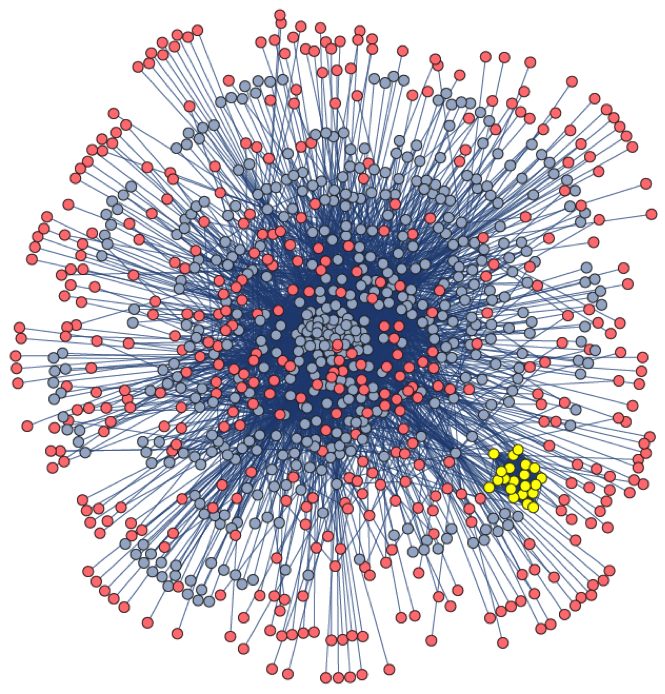
\includegraphics[scale=0.7]{IMG/LSPasd.png}
	\caption{Example Network of 1,000 nodes, MSM in yellow, women in red and men in blue.}
	\label{LSPnetwork}
\end{figure}


There are several types of networks of interest for the applied sciences. If we classify them according to the degree of a node, i.e., to the number of links for a given node (or, more properly, to the distribution of these number of links), we have two main categories in the literature: (i) random networks, in which the links or edges occur with a fixed probability and the statistical distribution of this number of links follows a Poisson's law; (ii) scale-free networks whose distribution of degrees follows a power-law with an algebraic tail of the form $P(k) \simeq 1/k^\gamma$ with $2 < \gamma < 3$. This means that the nodes with very large degrees are more likely to appear in scale-free networks than those in random networks. Random networks have been used in epidemiology \cite{acedo2011using} and also as an elementary model of the brain \cite{acedo2013brain}. On the other hand, scale-free networks have been successfully applied to the Internet and biological networks in which some nodes with a very large number of links are determinant in the control of the dynamics (see \cite{dorogovtsev2013evolution}) and (iii) small-world networks referring to the average length of a path connecting two typical nodes in the network. Small-world networks are an important paradigm in the science of networks. It was found that some sparse networks may present the small-world phenomenon, i.e., there are short paths connecting every pair of nodes through the links with other nodes. A mechanism to generate these networks was discovered by Watts and Strogatz \cite{watts1998collective}. Many networks in sociology exhibit this small-world property \cite{christakis2007spread,liljeros2001web,bearman2004chains}.

STD are more likely to produce large-scale infections than other transmissible diseases, such as respiratory transmitted diseases, because the efficacy of sexual contacts for the infection is large and the infectious agent has long latency periods as in the case of HIV or HPV. Moreover, neither the carrier nor his/her partner are aware of their exposure. For example, it has been estimated that around $40-50\%$ of contacts are capable of transmitting HPV \cite{burchell2006modeling}.

In order to predict the evolution of these diseases we need a reliable model of the underlying social network in which the infection builds up. Individuals who change partners or have several partners simultaneously, are the hubs favoring the spread of STD. The distribution of degrees of the nodes in the network and the average chemical path from an infected individual to a susceptible one, are important parameters controlling the final extension of a new STD in a population and the speed at which it spreads. However, most models are based on some assumptions, which could not be valid for certain populations. Some studies claimed that the web of human sexual contacts is a scale-free network characterized by a power-law distribution for the number of individuals with a certain degree of connectivity, $k$: $P(k)\propto 1/k^\alpha$ with a value of $\alpha$ in the range $2 <\alpha < 3$, and slightly smaller for males than for females \cite{liljeros2001web}. Although $P(k)$ provides some valuable information about the network, it is not a sufficient prescription on how to build it for a given population size. Moreover, a power-law distribution of contacts could not be representative of some populations, or could vary from country to country. For example, it has been found that a densely connected core appears without the need of a high connectivity degree in the Jefferson High School's network \cite{bearman2004chains}. 

Even with the high prevalence of STDs there are few studies devoted to ascertain the structure of sexual networks and its role in disease transmission. Most studies are restricted to small communities such as the Jefferson High Schools project \cite{bearman2004chains} or that of Likoma Island \cite{helleringer2007sexual}.

Some field studies have ascertained the structure of moderate size real networks of sexual contacts. In $2004$, Bearman et al. published the results for a set of $800$ adolescents in a mid sized town of the United States \cite{bearman2004chains}. They  showed that the structure of this network is a big cluster with a ring and extended filaments which contained most of the adolescents implying that, potentially, the infection of an individual could spread to the whole of the population, given sufficient time and infectivity. A similar study was performed in $2007$ at the Likoma Island in Malawi with the idea of predicting and explaining the expansion of HIV in sub-Saharan populations \cite{helleringer2007sexual}. That study disclosed  that the sexual network contained many cycles, in contrast with the single cycle at Jefferson High School. For that reason, it was speculated that superimposed cycles could be the explanation of the high prevalence of HIV infection in small populations of Africa.

Some recent studies reveal that the evolution of partnerships is also an important factor in the transmission of STDs. In particular, they pointed out that the following items should be considered: (i) the cumulative distribution of the lifetime number of partners, (ii) the distribution of partnership duration, (iii) the distribution of gap lengths between partnerships, and (iv) the number of recent partners. A method for building up networks considering these items has been developed by Schmid and Kretzschmar \cite{schmid2012determinants}. However, this information is not available in most surveys, and we therefore face the problem of developing reasonable models for STDs in many countries where information about sexual behaviour is scarce. For example, in the case of Spain, there is only available data about the number of sexual contacts in a lifetime from surveys. This is sufficient for building a sexual network for the transmission of HPV or other diseases with lifetime consequences and progression. In these cases, the important fact is whether the individual has had a contact with risk of infection. The remaining aspects of the network such as the duration of partnership and the time intervals among them can be incorporated effectively into a probability of transmission parameter.

%Network models are those models in which the relations of the individuals (represented by network sites) are taken into account by means of the network bonds. Random network models have been successfully applied to other infectious diseases such as the Respiratory Syncytial Virus pandemic \cite{acedo2011using} as well as other social pandemics such as obesity \cite{christakis2007spread}.

%Recuerda que el esfuerzo de construir el modelo de redes es porque se está observando que hay resultados del efecto de la vacuna mucho antes de lo que decía el modelo existente (Elbasha et al.), la aparición del debate de la vacunación de niños, que el modelo de Elbasha et al. no aporta mucho y que dicho modelo no explica bien el efecto comunitario. Esas cosas no las he visto claramente en la introducción.
\section{Our proposal}

In recent studies \cite{ali2013genital,fairley2009rapid} a decrease on the number of infected persons and the number of persons with GW is already reported for Australia after two years of administering vaccinations to young girls. It showed both direct and indirect prevention in males. These results were more impressive than the predictions of the continuous models. New vaccination schedules, specially vaccination in boys, should take into account the herd immunity effect vaccination in girls (in mainly heterosexual societies). 

A Bayesian model for HPV vaccination was then proposed by Bogaards et al. \cite{bogaards2015direct} and focused on the herd immunity effect of the female vaccination on the male population in a static picture. A dynamic understanding for the short and long term effects of vaccination policies is, however, still necessary and even more so with HPV vaccines because their benefit to the whole population is to be observed in the time span of several decades.

In this dissertation we propose a model based upon a network instead of traditional continuous models. We show how to build a network model for sexual contacts from the usual statistical data in surveys concerning the number of partners in a lifetime. We consider both heterosexual men and men who have sex with men (MSM) populations and the connections among them. We perform simulations over this network substrate on the HPV infections by different genogroups including both LR and HR infections. We will be able to determine with higher accuracy the effect of vaccination in a short and large periods of time, this is, the herd immunity effect. In particular, we show that for the case of Australia the strategy of a vaccination for $12-13$ year-old girls plus catch-up lead to a considerable reduction in the number of cases of infection by HPV 6 and/or 11 (which are the main cause of GW). For women in the $14-26$ age-group we obtain a decrease of $59\%$ after $3.6-4.6$ years and $39\%$ in men after $3-3.75$ years. These results agree with the conclusions of the study by Ali et al. \cite{ali2013genital}.

In the following chapters we will explain in detail: 
\begin{itemize}
	\item the building of the network model for sexual contacts. This is a technical-computational chapter;
	\item how the calibration of the model is carried out. This is a technical-computational chapter;
	\item model validation simulating the Australian scenario and obtaining similar results;
	\item the study of the decline of warts with the current vaccination campaign in Spain: vaccination of girls with a coverage of $70\%$;
	\item the study of the decline of oncogenic HPV with the current vaccination campaign in Spain;
	\item the study of what would happen if the effect of the vaccine disappear suddenly after $20$ years;
	\item the study to determine if the tourism in Spain has a significant effect on the HPV infection;
	\item the study of the decline of oncogenic HPV if we vaccinate boys and girls with a high coverage;
	\item the study of how long the decline is recovered after a drop in the coverage;
	\item the study of how the decline of HPV is affected when the average number of LSPs increases significantly;
	\item the study of how the decline of HPV is affected when the number of MSMs increases significantly.
\end{itemize}


